\begin{subsection}{Preparación}
  En esta sección se describe como se prepara el entorno de pruebas con los elementos y servicios utilizados para realizar el despliegue de la solución y necesarios para su correcto funcionamiento.

  \begin{subsubsection}{VMware Lab Constructor v4.0.1}
    El programa VMware Lab Constructor v4.0.1 (VLC), es una herramienta desarrollada por trabajadores de VMware, la cual permite crear un entorno embebido dentro del host utilizado como entorno de pruebas. Este entorno se compone de cuatro hosts con el hipervisor ESXi en forma de VMs. Dentro de estos hosts, VLC despliega los componentes de VCF.

    \begin{figure}[h!]
      \centering
      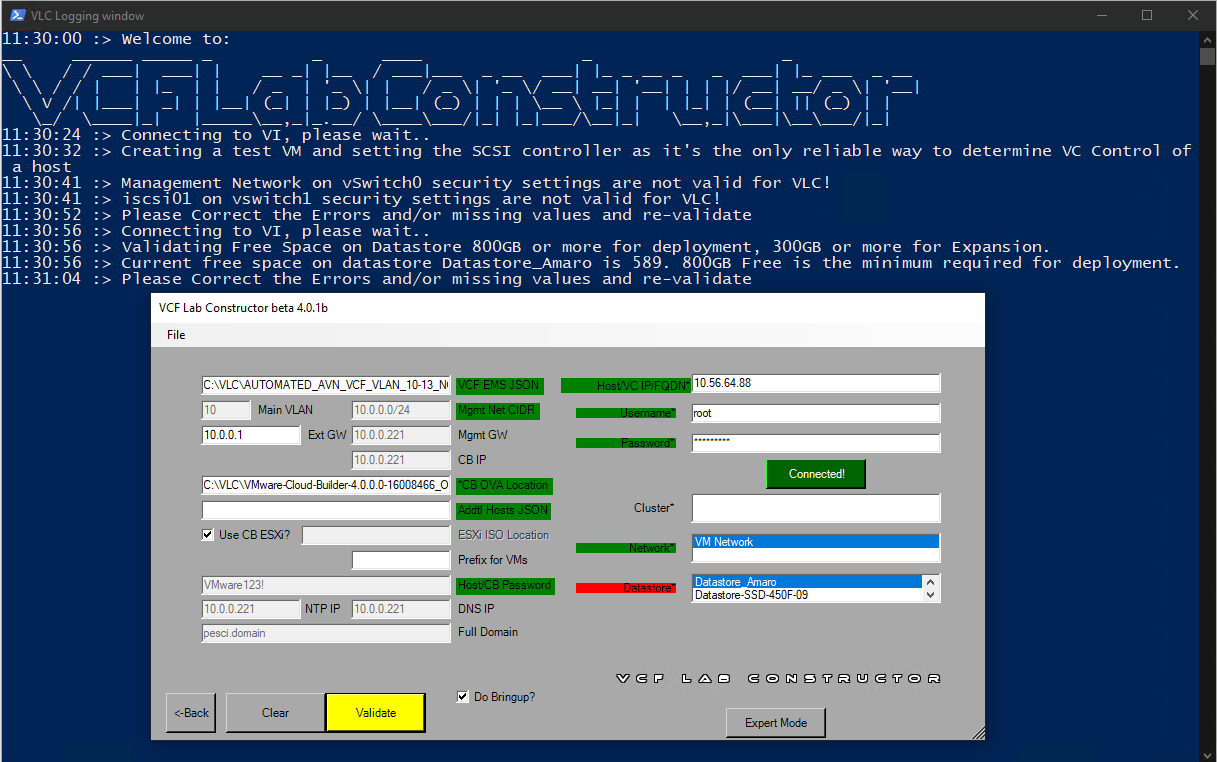
\includegraphics[width=0.8\textwidth]{imaxes/pruebaconcepto/VLC.png}
      \caption{Herramienta VMware Lab Constructor v4.0.1b}
      \label{fig:VLC}
    \end{figure}
    \FloatBarrier

  \end{subsubsection}

  \begin{subsubsection}{Host ESXi}  
    El host sobre el que VLC realiza la instalación del entorno se trata de un servidor con el hipervisor ESXi instalado. Este servidor cuenta con una memoria RAM de 192 GB, una CPU de 28,8 GHz y está conectado a un datastore formado por discos SSD y con una capacidad de 3 TB. Además, incorpora dos interfaces de red. La primera interfaz se conecta a una red para acceder al datastore, mientras que la segunda, representada con el nombre \textit{vmnic0} en la figura \ref{fig:estructura-generada-por-VLC}, se conecta a una red utilizada para acceder de forma remota al servidor y a otra red dedicada a comunicar los componentes desplegados dentro del host.

    % Como base para la instalación se utiliza un servidor físico con el hipervisor ESXi instalado. Este host se utiliza para desplegar los componentes de VMware Cloud Foundation para crear un pequeño SDDC embebido para probar sus funciones. Este host cuenta con una memoria RAM de 192 GB, una CPU de 28,8 GHz y un \textit{datastore} con discos SSD con 2 TB de capacidad. Cuenta con dos interfaces físicas, una que conecta al host con el \textit{datastore} y otra a la que se conectan dos redes, una llamada \textit{Management Network} que permite acceder al host desde una VM para gestionarlo, y otra llamada \textit{VM Network} donde se conectan todas las VMs generadas por VLC y de los servicios que dan soporte a los componentes de VMware Cloud Foundation.
  \end{subsubsection}

  \begin{subsubsection}{Servicios}
    Los servicios externos requeridos por VCF se sitúan dentro del mismo servidor físico. Estos están colocados en una VM con el sistema operativo Windows Server 2016, el cual incluye DNS, NTP, SMTP, y los servicios Active Directory (AD) y Certificate Authority (CA). También incorpora un router en forma de VM con el sistema operativo VyOS, que además cuenta con servicio DHCP. El servidor DNS utiliza \textit{pesci.domain} como nombre de dominio. El almacén Active Directory sustituye al directorio de usuarios de la UDC para poder manejar cuentas de usuarios sin causar conflictos en el funcionamiento de los servicios en producción.
    % Todos los servicios requeridos por VMware Cloud Foundation se despliegan sobre el mismo servidor en forma de VMs. Una de las VMs es Windows Server 2016 que contiene un servidor DNS, un servidor NTP, un servidor Active Directory, un servidor SMTP y ejerce también como Certificate Authority. Otra VM contiene el sistema operativo VyOS que funciona como un router virtual y como servidor DHCP. Una última VM con Windows 10\footnote{Se refiere a ella como \textit{Jump Host}.} se requiere para ejecutar VLC y acceder al entorno embebido generado por VLC.
    % El servidor DNS contiene el nombre y su respectiva dirección que un componente de VCF utilizará para que sus instancias se puedan comunicar con otras. Este servidor DNS implementa un único dominio que se denomina \textit{pesci.domain}. El servidor Active Directory proporciona un almacén de usuarios y grupos de usuarios a los cuales se les configura un rol dentro de cada componente de SDDC. Se utiliza este repositorio de usuarios en lugar del directorio real de la UDC para evitar posibles problemas del servicio. El router VyOS tiene configuradas todas las subredes y VLANs que VMware Cloud Foundation utiliza en la capa L3 de la infraestructura física y proporciona acceso a Internet, en las cuatro interfaces que conectan con las instancias de VMware NSX-T Edge utiliza enrutamiento dinámico BGP. El servidor DHCP se utiliza para asignar una dirección IP a las interfaces Tunnel EndPoint (TEP)\footnote{Más adelante se describirá la función de este elemento} de cada host ESXi.    
  \end{subsubsection}
  \begin{figure}[h!]
    \centering
    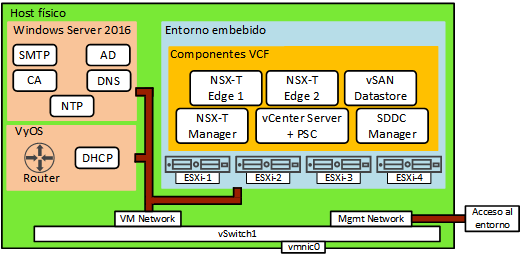
\includegraphics[width=0.6\textwidth]{imaxes/pruebaconcepto/hostFisico.png}
    \caption{Finalización del despliegue inicial de VMware Cloud Foundation.}
    \label{fig:fin-despliegue}
  \end{figure}
  \FloatBarrier
    \begin{figure}[h!]
      \centering
      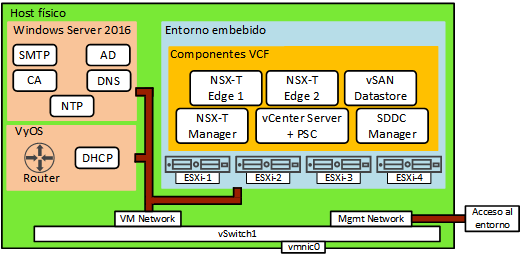
\includegraphics[width=0.8\textwidth]{imaxes/pruebaconcepto/hostFisico.png}
      \caption{Servicios desplegados y entorno embebido generado por VLC dentro del host físico.}
      \label{fig:estructura-generada-por-VLC}
    \end{figure}
    \FloatBarrier
    Una vez finalizado el despliegue como se muestra en la figura \ref{fig:fin-despliegue}, el entorno embebido generado con VLC dentro del host físico, incluyendo las VMs de los componentes de VCF y los servicios necesarios para su correcto funcionamiento, se muestra en la figura \ref{fig:estructura-generada-por-VLC}. Esta figura también incluye las dos redes a las que se conecta la interfaz \textit{vmnic0} del host. \textit{VM Network} comunica a todos los elementos desplegados y representa la red física del entorno. La red \textit{Mgmt Network} se utiliza para acceder al host de forma remota.
    % \begin{figure}[h]
    %   \centering
    %   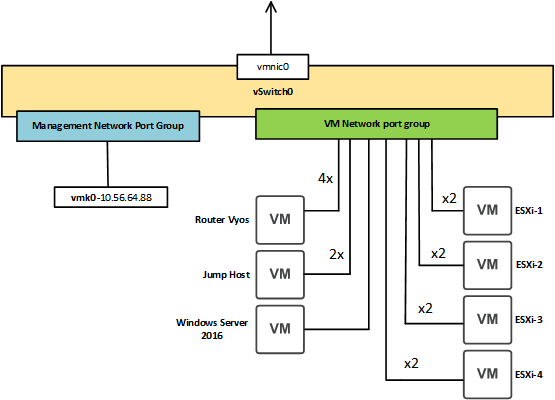
\includegraphics[width=0.6\textwidth]{imaxes/pruebaconcepto/vSwitch0HostFisico.png}
    %   \caption{Máquinas virtuales en el host físico.}
    %   \label{fig:VMs-alojadas-host-fisico}
    % \end{figure}
    % \FloatBarrier

    % En la imagen anterior se muestran las VMs que están funcionando sobre el host físico y que representan los componentes de la infraestructura física de un SDDC real, junto con el número de interfaces que se utilizan en cada una. Cada host ESXi generado por VLC cuenta con dos interfaces de red. El router VyOS, Jump Host y Windows Server 2016 se configuran antes del despliegue de VMware Cloud Foundation con VLC y se comunican con el entorno generado por VLC a través del \textit{port group} VM Network. El \textit{port group} Management Network se utiliza para acceder a la configuración del host físico a través de la dirección IP que se indica. Se utiliza la interfaz vmnic0 del host como salida del tráfico generado por el vSwitch0.
    % \FloatBarrier

    % \begin{figure}[h]
    %   \centering
    %   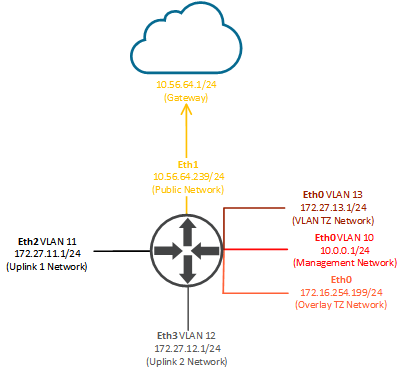
\includegraphics[width=0.4\textwidth]{imaxes/pruebaconcepto/RouterFisicoL3.png}
    %   \caption{Interfaces del router Vyos.}
    %   \label{fig:interfaces-router-fisico-L3}
    % \end{figure}
    % \FloatBarrier

    % En la imagen anterior se muestra la configuración del router VyOS. Cada una de las interfaces se debe configurar antes del despliegue de VCF. Todas usan MTU de 9000 Bytes ya que la mayoría de componentes de VCF utilizan paquetes de red \textit{jumbo frame}. En las interfaces Eth2 y Eth3 el router utiliza enrutamiento dinámico BGP donde el AS local es 65001 y el AS remoto es AS 65003, configurado para anunciar a sus vecinos la red 10.0.0.0/24 Management Network. Las direcciones configuradas como \textit{neighbour} son: 172.27.11.2, 172.27.11.3, 172.27.12.2 y 172.27.12.3. En la dirección IP 172.27.254.199 de la interfaz eth0, el router proporciona un servidor DHCP que asigna direcciones IP en el rango 172.16.254.0 - 172.16.254.100.
    % \FloatBarrier

    % \begin{figure}[h]
    %   \centering
    %   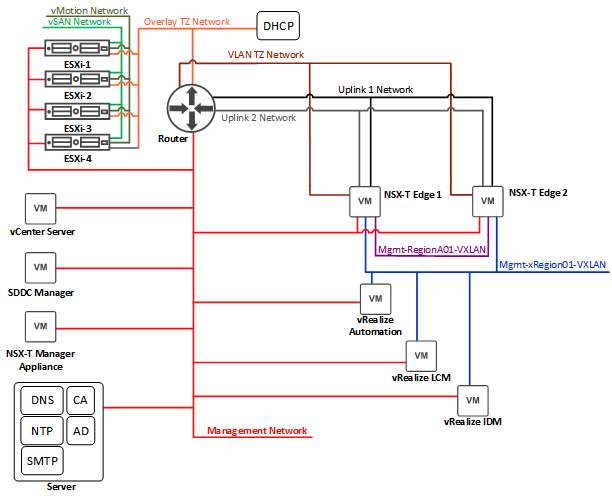
\includegraphics[width=0.6\textwidth]{imaxes/pruebaconcepto/RedDesdeDentro.png}
    %   \caption{Topología de las redes del entorno desplegado.}
    %   \label{fig:red-L3-infraestructura-fisica}
    % \end{figure}
    % \FloatBarrier

    % En la imagen anterior se muestran todos los componentes de VMware Cloud Foundation desplegados por VLC y los desplegados posteriormente para completar los objetivos del proyecto, como se conectan con los distintos servicios de red y a que redes se conectan. Las redes Mgmt-xRegion01-VXLAN y Mgmt-Region01A-VXLAN se corresponden a redes virtuales gestionadas por VMware NSX-T que no requieren ninguna configuración adicional en la capa 3 de la infraestructura física (esto se verá con detalle en el apartado de diseño de VMWare NSX-T).
    % \FloatBarrier
  

    


    
    
    
  \end{subsection}